\chapter{Attaques et défenses}


% esquives


\section{Attaque}
\label{sec:att-def:attaque}


\subsection{Concepts généraux}


\begin{definition}[Attaques simple et composée]
\index{attaque}

\noindent
On peut distinguer les attaques simples des attaques composées :
\begin{itemize}
	\item une \emph{attaque simple} consiste en un coup isolé ;
	\item une \emph{attaque composée} (ou technique) est une séquence d'actions, chacune ayant pour objectif de préparer la suivante.
\end{itemize}
\end{definition}


Le principal intérêt d'une attaque simple est de tester l'adversaire (type de réaction, temps de réponse…) ou de le faire réagir (forcer un changement de garde…).
Des attaques simples peuvent être enchainées sans pour autant former une attaque composée : par exemple on peut induire un schéma en attaquant alternativement à gauche et à droite avec des coups de taille, pour ensuite le briser et surprendre l'adversaire.

Une attaque composée se distingue d'une attaque simple principalement par l'intention : chaque composante de l'attaque est différente et permet de préparer le terrain.
L'exemple le plus simple d'une attaque composée est une feinte sur une cible suivie d'une attaque sur une autre ouverture : si la feinte est crédible l'adversaire cherchera à se défendre contre la première attaque ce qui ouvre une autre ligne, et du fait que l'attaquant ne porte pas son coup jusqu'au bout il dispose d'une avance (en plus de l'effet de surprise).
L'idée générale est de placer l'opposant dans une situation qui le forcera à réagir d'une manière que nous pouvons exploiter : en effet face à une situation donnée il existe un certain nombre de réactions possibles (conditionnées en partie par l'arme, le style et l'expérience).
Cela explique l'intérêt d'apprendre des techniques : on dispose alors d'un vaste répertoire de pièces que nous pouvons exécuter afin de prendre l'avantage, que nous ayons pris l'initiative ou non à l'origine.
Toutefois il faut être prêt à changer son plan si l'adversaire ne réagit pas comme prévu ou si l'on perçoit une opportunité : ainsi si l'on veut exécuter une feinte mais que l'adversaire ne se protège pas alors il faut porter la frappe jusqu'au bout.

% TODO: changer de section ?

Une attaque s'accompagne d'un mouvement de jambes qui permet de donner plus de force au mouvement et de sortir de l'axe (définition~\ref{dep:def:sortie-axe}).
En effet si l'attaque se fait en avançant droit devant il y a le risque d'un coup double si l'adversaire fait de même.


\begin{coup}[Attaque normale]
\index{coup}
\index{attaque|see{coup}}

Partant d'une garde avec le pied droit (resp.\ gauche) en arrière, l'attaquant porte un coup depuis son côté droit (resp.\ gauche) en avançant le pied droit (resp.\ gauche).
\end{coup}

Le fait que le pied et l'attaque ait lieu du même côté s'expliquer par le fait que le coup est plus puissant de cette manière : dans le cas contraire, appeler contre-pied, le mouvement n'est pas naturel pour le corps (voir le commentaire dans Ringeck~\cite[p.~7]{farrell:ringeck}).
Toutefois il peut arriver que l'on souhaite attaquer du côté où se trouve le pied avant (par exemple redoubler une attaque) : dans ce cas on effectuera quand même un déplacement des pieds accompagné d'une sortie d'axe.
À noter aussi que pour certaines armes, comme l'épée longue~\cite[p.~10]{farrell:ringeck}, il est conseillé d'attaquer en premier du côté dominant car on pourra y mettre plus de force : ainsi un droitier devrait commencer par attaquer à droite, et inversement pour un gaucher.

\index{prise}
Lorsqu'une attaque est exécutée il faut veiller à ne pas casser le poignet : l'arme et le bras doivent former ensemble un angle droit (figure~\ref{attdef:fig:poignet-cassé}).
On pourrait avoir l'impression que casser le poignet permet de gagner en allonge, mais en réalité cela cause plusieurs problèmes importants :
\begin{itemize}
	\item lorsque le poignet est cassé nous ne pouvons pas mettre de la force dans l'arme et l'adverse peut la contrôler plus facilement ;
	
	\item cela augmente les risques de blessure, à court et long termes ;
	
	\item la position est moins hermétique et l'adverse dispose de plus de cibles.
\end{itemize}
En effet placer le poignet en extension n'est pas une position naturelle (a fortiori en tenant une arme d'un kilogramme), et on sent très vite que l'on ne peut pas garder cette position longtemps.
Ainsi que nous l'avons vu dans les chapitres précédents toute position inconfortable indique qu'il faut changer quelque chose.


\begin{figure}[ht]
	\centering
	\subfloat[Prise correcte.]{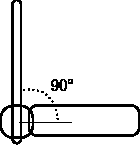
\includegraphics[scale=1]{structure/prise_poignet_correct.pdf}}
	\hspace{3cm}
	\subfloat[Poignet cassé.]{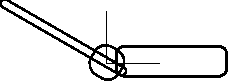
\includegraphics[scale=1]{structure/prise_poignet_casse.pdf}}
	\caption{Comparaison entre une prise correcte et une prise avec le poignet cassé.}
	\label{attdef:fig:poignet-cassé}
\end{figure}


Une attaque doit viser une cible précise : il n'est pas question d'agiter son épée au hasard en espérant obtenir quelque chose, d'autant plus que cela est dangereux dans le cadre de la pratique sportive.
Ainsi il peut être utile de s'arrêter par moment afin de vérifier que la cible visée a bien été atteinte.
La cible est assimilée à un point dans l'espace : si l'opposant se déplace pour éviter l'attaque il ne faut pas chercher à le suivre (sauf si cela fait partie de la technique), sinon on lui permet de nous amener là où ile décide.
De plus une fois que l'on a atteint la position visée il ne faut pas continuer la coupe jusqu'au bout, car alors on se prête à une riposte : après chaque attaque il faut absolument se retrouver dans une garde qui ne laisse aucune ouverture.
L'adversaire doit être gêné par la position de notre arme après la frappe.
Ainsi que cela a été mentionné plus haut cela implique de ne pas casser le poignet.

% cf escrime japonaise

L'attaque à contre-pied va à l'opposé de l'attaque normale telle qu'elle a été décrite plus haut.
Elle permet de gagner en distance et de surprendre l'adversaire.
Le gain de distance par rapport à la position normale est due à la position des épaules.

\begin{coup}[Attaque à contre-pied]
\label{struct:coup:contre-pied}
\index{coup!en contre-pied}
\index{contre-pied}

Une attaque à contre-pied consiste à avancer le pied du côté opposé à celui où l'on attaque.
\end{coup}


\subsection{Cibles}


Les cibles précises dépendent de l'arme considérée mais il existe certaines idées générales.
Une cible intéressante est ouverte : cela signifie que l'adversaire ne la protège pas et qu'il va lui falloir un temps de réaction avant de pouvoir le faire.
L'idée générale est donc de créer une ouverture, en conduisant l'adversaire à ne pas protéger une partie de son corps que l'on peut ensuite attaquer.


\begin{definition}[Ouverture]
\index{ouverture}

Une ouverture correspond à une cible qui n'est pas protégée (au moment où l'attaque est initiée).
\end{definition}


On distingue entre les cibles hautes et basses selon leur position : les premières regroupent la tête, le torse et les bras, les secondes les jambes et le bas du torse.
Il est évident que la tête est une cible importante, mais il peut être beaucoup plus intéressant de viser le torse -- plus grande superficie -- ou les membres (appelés aussi avancées) -- plus faciles à atteindre.
Pour cette raison il est important de toujours s'assurer que l'avant-bras ne peut pas être facilement atteint par l'adversaire à chaque fois que l'on attaque (en particulier si l'on dispose d'un bouclier celui-ci doit couvrir le bras).
En effet il suffit d'une blessure suffisamment importante au bras d'arme pour empêcher l'adversaire de continuer le combat : dans ce cas il n'y a aucune raison logique de vouloir viser absolument la tête ou le torse.
Comme nous en avons déjà parlé dans l'introduction le point clé est de mettre fin au combat le plus vite possible -- en survivant.
Attaquer le bras est particulièrement intéressant car si l'on se trouve juste à portée pour frapper le bras cela signifie que nous sommes hors distance par rapport à l'arme de l'opposant (si les armes sont similaires).


\begin{definition}[Cibles basse et haute]
\index{cible!basse}
\index{cible!haute}

Une cible est dite haute/basse si elle se trouve au-dessus/en-dessous de la ceinture (nombril).
\end{definition}


\begin{coup}[Attaques aux avancées]
\index{attaque!aux avancées}

Une attaque aux avancées consiste à attaquer le bras (ou parfois la jambe) de l'adversaire, en général suite à une attaque de celui-ci.

\end{coup}


% TODO: améliorer
\begin{exercice}[Attaques aux avancées]

\begin{enumerate}
	\item \A porte une attaque simple sur \D et arrête le coup avant la touche.
	
	\item \D vérifie s'il peut facilement blesser \A au bras.
\end{enumerate}

L'exercice peut être modifié, par exemple en permettant à \D de se protéger ou d'esquiver (avec un pas), ou bien en n'autorisant \D à toucher \A que s'il se trouve en sécurité.

\end{exercice}


% TODO: jeu de 8 cibles
% TODO: jeu complet


\subsection{Compléments}


Le fait de passer d'une prise en pronation à une prise en supination (ou inversement) tout en gardant la main au même endroit permet de changer la ligne d'attaque.
En particulier cela peut permettre de placer l'épée pour blesser l'adversaire tout en restant soi-même protéger : en effet si l'arme est tournée vers l'extérieur dans la position initiale, le changement pronation/supination permet d'effectuer une rotation de \ang{180} et de passer derrière la garde adverse.


\begin{technique}[Changement de ligne]
\label{struct:tech:changement-ligne}

\A et \D ont les lames en contact, la garde est prise à droite en pronation.
\A tourne sa main en supination afin de passer sa lame derrière celle de \D pour le toucher.

% Source : Romain.
\end{technique}


\section{Défense}


% dévier/absorber, parade franche, esquive (avec/sans couverture), reculer


\section{Concepts}


% temps
Un certain nombre de paramètres entrent en compte



\subsection{Distance}


La distance est un concept important car les techniques utilisées vont varier en fonction de celle-ci.
De plus il faut s'habituer à être capable d'évaluer rapidement les différentes distances en fonction de l'arme utilisée : être hors distance ne signifie pas la même chose quand on se bat à mains nues ou avec une lance.

Dans la définition ci-dessous nous indiquons entre parenthèses le nom allemand correspondant~\cite{kronenburg:dijon:going_distance:2015}.
L'attribution de ces mots est sujette à débat mais nous les donnons car certains les utilisent.
"Ringen" signifie "corps-à-corps", "arm" signifie "bras" et "leib" signifie "corps".
% cf Forgeng Glossary

\begin{definition}[Distances]
\index{distance}

\noindent
La distance entre deux opposants peut être définie selon les actions possibles :
\begin{itemize}
	\item \emph{hors distance} : les deux combattants sont éloignés et ne peuvent mener aucune action offensive directement ;
	
	\item \emph{approche} (zufechten) : les deux combattants sont éloignés et il suffit d'un temps pour arriver au contact des lames ;
	
	\item \emph{engagement} (fechten) : les armes des deux combattants peuvent se toucher, mais ils sont trop éloignés pour pouvoir toucher directement l'autre ;
	
	\item \emph{engagement proche} (kriegen) : les armes des deux combattants peuvent se toucher et l'opposant est à distance de touche ;
	
	\item \emph{combat rapproché} (armringen) : les deux opposants sont suffisamment proches pour pouvoir toucher l'autre en tendant le bras ou la jambe ;
	
	\item \emph{corps-à-corps} (leibringen) : les deux opposants sont très proches et peuvent travailler sur tout le corps de l'adversaire.
\end{itemize}
\end{definition}


\begin{definition}[Jeux long et court]
\index{distance!jeu court}%|textbf
\index{distance!jeu long}
\index{jeu|see{distance}}

\noindent
En escrime italienne les distances sont rassemblées de la manière suivante :
\begin{itemize}
	\item \emph{jeu long} : hors distance, approche, engagement ;
	
	\item \emph{jeu court} : engagement proche, combat rapproché, corps-à-corps.
\end{itemize}
\end{definition}

% À l'épée longue le jeu court est caractérisé par la position de \emph{mezza spada}, où les deux armes sont au contact au milieu de la lame.

La division du combat en six distances est relativement arbitraire et les frontières sont parfois floues, selon les armes et les styles.
Toutefois cela donne une première idée des actions possibles en fonction de la distance et peut servir de base au raisonnement.

Un combat débute typiquement avec les adversaires hors distance : plusieurs temps sont nécessaires avant de pouvoir lancer une attaque.
Il s'agit d'une phase d'observation où chacun essaie de se faire une idée de son opposant.
Pour cette raison les positions de garde sont peu offensives et défensives : on privilégiera des positions reposantes car l'adversaire est trop loin pour surprendre.
Il peut arriver pendant un combat que les adversaires s'éloignent pour se mettre hors distance afin de souffler.

La position devient plus hermétique dans la phase d'approche : l'adversaire est capable de porter rapidement un coup et il faut être prêt à réagir vite.
Dès qu'une attaque est portée on arrive à l'engagement : les armes sont généralement au contact afin de contrôler les mouvements de l'adversaire et de \emph{sentir} l'intention de l'adversaire.

Dès que l'engagement se rapproche il devient possible de blesser directement l'adversaire et il est donc important de ne pas perdre le contrôle et de ne pas laisser d'ouverture.
On commence aussi à disposer d'un manœuvre plus large sur l'arme de l'adversaire.
% escrime allemande
À noter que l'on passe souvent de la phase d'approche à la phase d'engagement rapproché directement : il suffit que la cible lors de l'attaque soit le corps de l'adversaire pour se retrouver très proche à la fin de l'attaque.

Finalement le combat rapproché permet de donner des coups de poing et de pied à l'adversaire.
En outre on se trouve suffisamment proche pour exécuter certaines clés sur les bras, typiquement.
Le corps-à-corps constitue la dernière étape du combat, et peut éventuellement se dérouler au sol : elle contient des saisies et des clés sur tout le corps (étranglements…) et des projections.



\subsection{Temps}




\subsection{Sentiment du contact}


\index{sentiment du fer}
Le sentiment du contact, aussi appelé plus spécifiquement le sentiment du fer, consiste à sentir l'intention de son adversaire à travers le contact que l'on a avec lui, que ce soit via les armes (bouclier compris) ou le corps.


\begin{exercice}[Variante à l'échauffement d'Ingulf]
\label{att:ex:Ingulf-variantes}
\index{echauffement@échauffement!exercice}

\obj{Cet exercice travaille la structure, l'équilibre et le sentiment du contact.}

La disposition initiale est identique à celle de l'exercice~\ref{struc:ex:Ingulf}.
Lors du déplacement des actions supplémentaires peuvent être exécutées par \A et \D afin de travailler le sentiment du contact :
\begin{enumerate}
	\item Changement de garde : \A peut passer le bras à l'extérieur (gauche au début de l'exercice) sous le bras de \D pour venir attraper l'intérieur de son coude droit.
	Cela met \A dans une position avantageuse car il contrôle totalement le centre et oblige \D à se retrouver de face, avec les deux bras à l'extérieur.
	Au combat \D possèderait peu de cibles intéressantes, à l'opposé de \A.
	
	Afin de ne pas se retrouver en position dominée \D a intérêt à changer lui aussi de garde en même temps que \A, afin de rétablir l'équilibre.
	Dans ce cas la position est exactement opposée à celle de départ.
	
	\item \A essaie d'attraper le bras de \D.
	Pour ce faire il doit lâcher sa prise et passer ses deux bras sous le bras de \D afin de le plaquer contre sa poitrine avec ses avant-bras.
	Attention aux pouces !
	L'objectif de \D est de sentir le moment où \A lâche son autre bras afin de retirer le bras ciblé.
	
	En explorant on peut remarquer que deux moments sont particulièrement adaptés : quand \D change de garde et quand \D pousse vers l'avant.
	
	\item Si \A essaie d'attraper le bras et que \D parvient à se retirer alors \D essaie de se placer dans le dos de \A et de l'enserrer avec ses bras.
	
	\item \A peut lâcher une de ses mains afin de venir toucher la tête de \D.
	\D doit sentir à quel moment \A lâche sa main afin d'esquiver en se baissant.
	
	La difficulté se trouve dans le fait que \A, à ce point de l'exercice, \A peut lâcher sa main pour exécuter différentes actions et \D doit sentir son intention.
	
	\item Fermer les yeux.
\end{enumerate}
Ces divers éléments peuvent être ajoutés un par un (en particulier la première variante est simple et devrait être ajoutée rapidement).

\source{\cite{Kohlweiss:2014:Dijon:RingenSchwert}}
\end{exercice}


\section{Exercices}


Certains des exercices peuvent se faire en plaçant un banc entre les deux partenaires.


\subsection{Mains nues}


Les exercices suivants peuvent se faire en statique ou en se déplaçant.


\begin{exercice}
\label{struct:ex:contact:frappe-signal}

\A et \D sont en garde, avant-bras en contact.
Quand \A baisse sa main, \D vient frapper à l'épaule.

Source : Romain.

\end{exercice}


\begin{exercice}

\A et \D sont en garde, avant-bras en contact.
\A donne un signal, \D vient frapper à l'épaule en enroulant un peu le bras et en gardant le contact.

Source : Romain.

\end{exercice}


\begin{exercice}
\label{struct:ex:contact:frappe-épaules}

\A et \D sont en garde, avant-bras en contact.
Quand \A le sent, il tend le bras droit pour toucher \D sur une épaule (\D ne cherche pas à se protéger).

Naturellement \A peut toucher \D à l'épaule droite juste en tendant le bras.
Mais si \A est parvenu plus dans l'intérieur de \D (par exemple en se déplaçant sur le côté plus vite, ou après un quarté du pied), alors il peut venir le toucher à l'autre épaule.

\end{exercice}


\begin{exercice}
\label{struct:ex:frappe-gauche-droite}

\A et \D se font face.

\begin{enumerate}
	\item \A frappe l'épaule gauche de \D de la main droite, en avançant la jambe droite.
	\item \D vient couvrir avec son bras droit en tournant les hanches.
	\item \A avance la jambe gauche et pose sa main gauche sur l'épaule droite de \D, en maintenant le contact avec la main droite.
\end{enumerate}

Dans l'intérêt de l'exercice, \D ne doit pas avancer sur \A.
Cet exercice est utile pour préparer certains enchaînements d'attaque droite puis gauche (e.g.
en épée longue allemande).

\end{exercice}


\subsection{Armes}


Il est intéressant de varier les armes avec lesquelles sont faits les trois exercices suivants afin de s'entraîner à estimer les distances dans divers cas.
À chaque fois l'attaque doit être normale par rapport à l'arme utilisée (ni forcée, ni exagérée, etc.).
La croix de la garde d'une épée longue (en nylon) renversée peut servir de cible.


\begin{exercice}[Mouvement dans le vide]
Effectuer des attaques simples dans le vide, puis des enchaînements.

Cet exercice devrait être un des premiers à effectuer avec toute nouvelle arme afin de s'habituer à son poids, à sa taille, aux mouvements possibles avec le corps, etc.
\end{exercice}


\begin{exercice}
\A et \D choisissent une arme quelconque.

\begin{enumerate}
	\item \A avance et s'arrête quand il se juge juste hors distance d'une attaque de \D.
	
	\item \D porte l'attaque pour vérifier.
\end{enumerate}

Source : Romain.

\end{exercice}


\begin{exercice}
\A et \D choisissent une arme quelconque.

\begin{enumerate}
	\item \A avance et \D lui dit de s'arrêter quand il le juge juste hors distance.
	
	\item \A porte l'attaque pour vérifier.
\end{enumerate}

Source : Romain.

\end{exercice}


\begin{exercice}
\A choisit une arme quelconque.

\begin{enumerate}
	\item \D avance et \A lui dit de s'arrêter quand il le juge juste à portée d'attaque.
	
	\item \A porte l'attaque pour vérifier.
\end{enumerate}

Source : Romain.

\end{exercice}


\begin{exercice}
\label{ex:frappe-dist:approche-frappe}

\begin{enumerate}
	\item \A et \D démarrent hors distance.
	\item \D s'approche de \A.
	\item Quand \A pense qu'il est à la bonne distance, il porte une frappe.
\end{enumerate}

Le but de \A est de parvenir exactement à la bonne distance pour que sa frappe soit efficace, donc ni trop près, ni hors distance.
La frappe de \A peut se faire en avançant ou en se décalant sur le côté, selon le type d'arme.
Au début on peut choisir de faire pratiquer toujours la même frappe (e.g.
un oberhau), puis ensuite de laisser le choix.
Finalement il est possible d'utiliser la croix d'une épée en nylon pour donner une cible.

\end{exercice}


\begin{exercice}
\label{ex:frappe-dist:approche-double-frappe}

Suite de l'exercice~\ref{ex:frappe-dist:approche-frappe}.

\begin{enumerate}
	\item \A et \D démarrent hors distance.
	\item \D s'approche de \A.
	\item Quand \A pense qu'il est à la bonne distance, il porte une frappe.
	\item \D recule un peu et \A porte une nouvelle attaque.
\end{enumerate}

La seconde attaque peut être soit à gauche normalement (en changeant de pied), soit en contre-pied à droite.
\end{exercice}


\begin{exercice}
\label{ex:frappe-dist:approche-croix-aleat}

La croix d'une épée nylon sert de cible.

\begin{enumerate}
	\item \A et \D démarrent hors distance.
	\item \D s'approche de \A, et à un moment décide de placer son pommeau (plus ou moins tôt) vers l'une des quatre directions nord/sud/est/ouest.
	\item Quand \A pense qu'il est à la bonne distance, il porte deux frappes consécutives dans les deux angles.
\end{enumerate}

Source : Jan.

\end{exercice}


\begin{exercice}
\label{ex:frappe-dist:approche-croix-aleat-garde}

Même exercice que \ref{ex:frappe-dist:approche-frappe}, mais juste après son coup \A doit reculer tout en revenant en garde.

Pour y parvenir \A doit être prêt à se déplacer rapidement, donc il doit être fléchi et souple pour pouvoir enchaîner les deux actions.

Cet exercice aide à préparer le combat libre.

% combat libre
\end{exercice}


\begin{exercice}
\A se met en équilibre sur une jambe et pratique n'importe quel exercice de frappe sur cible fixe.

Dans cet exercice il est très facile de voir si \A utilise uniquement ses bras ou tout son corps pour porter ses frappes.
\end{exercice}


\begin{exercice}

\begin{enumerate}
	\item \D tient l'épée horizontalement et se déplace.
	
	\item \A vient couper dessus, en essayant d'être juste limite au niveau de sa pointe.
\end{enumerate}

Si \A réussit à toucher à chaque fois alors c'est trop facile.

Source : Romain.

\end{exercice}


\begin{exercice}
\A et \D n'ont aucune protection.

\A porte une attaque et touche \D (juste un contact léger), à ce moment \D attaque \A (sans s'être protégé), et ainsi de suite.

L'idée de l'exercice est de perdre la peur d'être touché par l'arme de son équipier tout en apprenant à gérer sa force et la distance.
\end{exercice}


\section{Résumé}


\noindent
Voici une liste des principaux concepts que nous avons vus au sujet d'une attaque correcte :
\begin{itemize}
	\item l'attaque se fait du côté du côté du pied qui avance ;
	\item ne pas casser le poignet ;
	\item ne pas suivre la cible.
\end{itemize}


% attaque au bras
